% Valid Is Not Manufacturable
% Build with:
%   pdflatex main && bibtex main && pdflatex main && pdflatex main
% (latexmk is not used: the MiKTeX install it was written on has no Perl.)
%
% Figures are regenerated from the corpus, never edited by hand:
%   python research/figuras_paper.py data/garmentcodedata_0 docs/paper/figs
%   python research/sensibilidad_umbrales.py data/garmentcodedata_0 docs/paper/figs
% Numbers quoted in the text: research/numeros_paper.py -> figs/numeros_texto.json
%
% Generic class on purpose: it compiles on a stock MiKTeX install with no venue
% template. Switching to a venue template only touches this preamble.

\documentclass[10pt,twocolumn]{article}

\usepackage{lmodern}   % scalable font: microtype needs it with T1
\usepackage[T1]{fontenc}
\usepackage[utf8]{inputenc}
\usepackage[english]{babel}
\usepackage{microtype}
\usepackage{booktabs}
\usepackage{graphicx}
\usepackage{amsmath}
\usepackage{listings}
\usepackage[numbers]{natbib}
\usepackage[hidelinks]{hyperref}
\usepackage[margin=2cm]{geometry}
\usepackage{xcolor}
\usepackage{array}
\usepackage{tabularx}

\graphicspath{{figs/}}

\newcommand{\todo}[1]{\textcolor{red}{[TODO: #1]}}
\newcommand{\hilvan}{\textsc{Hilv\'an}}

\lstset{
  basicstyle=\ttfamily\footnotesize,
  breaklines=true,
  columns=fullflexible,
  frame=single,
  framesep=4pt,
  xleftmargin=2pt,
  showstringspaces=false,
}

\newcommand{\code}[1]{\texttt{\small #1}}

\title{\bfseries Valid Is Not Manufacturable:\\
Auditing Generative Sewing Patterns at Corpus Scale}

\author{Camilo Cuello \\
\small Universidad Nacional de Colombia \todo{department, to confirm with the author} \\
\small\texttt{ccuello@unal.edu.co}}
\date{September 2026}

\begin{document}
\maketitle

\begin{abstract}
Generative models for garment design are judged on whether they emit a
well-formed sewing pattern; whether that pattern can be cut and sewn goes
unmeasured. We measure this gap on GarmentCodeData~\citep{gcdata}, the de facto pre-training corpus of
the field. Of 3{,}450 published patterns, all of which passed physical
simulation, 20.4\% carry a hard geometric defect, with edges as short as
0.018\,cm and corners as sharp as $0.12^\circ$. Another 69.1\% cannot be judged:
the format records which edges a seam joins but not why their lengths differ,
so an intended gather looks like a defect. We propose three minimal format
extensions that make this intent expressible, and \hilvan, an open-source,
deterministic validator that runs on a CPU in about 10\,ms per pattern.
Discarding every pattern with an error keeps 10.5\% of the corpus and halves
its share of full-body garments; discarding only hard defects keeps 79.6\% with
the composition intact. Body shape has no detectable effect on hard-defect rates
(paired McNemar $p = 0.91$, 2{,}953 designs), so the defects come from the
design program. Applied to AIpparel, the same measurement finds 23\% of
image-conditioned and 17\% of text-conditioned patterns free of hard defects,
against 78\% of the matching corpus patterns, at the same seam count (31.6
against 31.5); 88\% of the generated seams join edges of unequal length.
\end{abstract}

\section{Introduction}

Current generative fashion tools produce images, and turning one into a
pattern a factory can cut still requires a patternmaker. A parallel line of
work therefore targets the sewing pattern itself: the 2D panels, their boundary
curves, and the seams that join
them~\citep{garmentcode,chatgarment,aipparel,sewingldm}.

These systems are evaluated, implicitly or explicitly, on whether their output
\emph{parses}: panels close, the seam graph resolves, the generator returns
without raising. We call this property \emph{validity}. Industry needs a
stronger one, whether the pattern can be cut from fabric and sewn by a machine,
which we call \emph{manufacturability}. Validity does not imply it.
Section~\ref{sec:method} turns it into two measurable levels. A pattern is
\emph{hard-defect-free} when no panel has a geometric defect that no reading of
the file can excuse, and \emph{fully validated} when, in addition, every seam
length mismatch is declared.

An edge measuring 0.018\,cm cannot be cut, and a corner of $0.12^\circ$ cannot
be sewn without the fabric bunching. Two edges sewn together whose lengths
differ by 9\% will pucker, unless the difference is a gather the designer asked
for, in which case it is correct construction. The current representation has
no field that tells these two cases apart, so no validator built on it can
either.

\paragraph{Contributions.}
\begin{enumerate}\itemsep1pt
  \item A corpus-scale measurement with explicit definitions. On
  GarmentCodeData, 20.4\% of published patterns carry a hard geometric defect
  and 10.5\% are fully validated; the first figure holds under threshold sweeps
  and vertex merging (Sections~\ref{sec:res-gap} and~\ref{sec:res-robust}).
  \item Three minimal format extensions, for seam ease, edge finishing and seam
  orientation, with evidence that orientation cannot be inferred from the file
  and a corpus-scale measurement of the convention GarmentCode follows
  (Section~\ref{sec:intent}).
  \item \hilvan, an open-source validator with every threshold disclosed,
  including a 2D criterion for tangent continuity across seams and an account
  of how legitimate construction had to be recognized for the checks to be
  usable (Sections~\ref{sec:method} and~\ref{sec:calibration}). The name is
  Spanish for a basting stitch, the provisional seam sewn to check a garment
  before it is sewn for real.
  \item Empirical guidance for using such a validator: the zero-error filter is
  biased against complex garments while a defect-class filter is not
  (Section~\ref{sec:res-filter}); hard-defect rates do not depend on body shape
  (Section~\ref{sec:res-body}); and applied to AIpparel, the metric locates the
  failure in seam length agreement rather than in garment complexity or
  conditioning modality (Section~\ref{sec:res-gen}).
\end{enumerate}

\section{Background and Related Work}

\paragraph{Pattern representation.}
A sewing pattern is a set of flat panels whose boundary edges are joined by
seams. GarmentCode~\citep{garmentcode} expresses garments as parametric
programs over roughly 80 parameters, emitting a JSON pattern in which each
panel carries 2D vertices, edges with optional B\'ezier or circular-arc
curvature, a 3D placement, and a semantic label such as \code{arm} or
\code{torso}. Each seam is a pair of references $\{\textit{panel},
\textit{edge}\}$. GarmentCodeData~\citep{gcdata} scales this to roughly
115{,}000 synthetic garments, following an earlier synthetic dataset by the
same group~\citep{korosteleva2021}, and is the de facto pre-training corpus for
the models below. Graphics work has long used the pattern as the primary
object, parsing existing 2D patterns into 3D garments~\citep{berthouzoz2013} or
keeping a pattern and its drape consistent during interactive
editing~\citep{sensitivecouture}, and Textile IR~\citep{textileir} proposes an
intermediate representation between fashion CAD and physical simulation. The
extensions of Section~\ref{sec:intent} are narrower: they add the reason for a
length difference to the seam record of an existing format.

\paragraph{Generative models.}
Learned models reconstruct patterns from point clouds~\citep{neuraltailor} and
images~\citep{sewformer,panelformer}, and generate them from text or
multimodal input~\citep{dresscode,sewingldm,garmentdiffusion,garmentimage}.
Two families matter here. Parameter-emitting models predict the inputs of a
pattern program: ChatGarment~\citep{chatgarment} has a vision--language model
emit GarmentCode's parameter schema key by key, and
Design2GarmentCode~\citep{design2garmentcode} synthesizes GarmentCode programs
from design concepts, so their expressive ceiling is the program's space.
Geometry-emitting models predict the pattern itself. AIpparel~\citep{aipparel}
tokenizes geometry as drawing commands (\code{MOVE}, \code{LINE},
\code{CURVE}, \code{CUBIC}, \code{ARC}) with seams encoded as labels shared
between edges. This removes the parametric ceiling but offers no validity
guarantee, and its code defines error types for token sequences that fail to
decode~\citep{aipparelrepo}. Because seams are labels rather than constraints,
nothing ties the two edges they join to a common length. Section~\ref{sec:res-gen}
measures the consequence.

\paragraph{Validity in generative CAD.}
Generative CAD models report how often their output cannot be built.
DeepCAD~\citep{deepcad} reports the fraction of generated command sequences
that yield an invalid topology, and Text2CAD~\citep{text2cad} an invalidity
ratio. These rates correspond to our notion of validity. Design for
manufacture~\citep{boothroyd2010} asks a stronger question, whether a part can
be produced by a given process, and that is the question we ask of sewn
garments.

\paragraph{Checker-in-the-loop generation.}
Code generation has a mature pattern in which a cheap, deterministic checker
returns localized errors and the generator uses them: repairing programs from
compiler diagnostics~\citep{drrepair}, rewarding programs by unit-test
outcome~\citep{coderl}, reranking candidates with a verifier trained on
execution results~\citep{lever}, and prompting a model to debug its own output
from execution feedback~\citep{selfdebug}. Our findings carry the panel, edge
or seam reference and the measured values for this use. What sewing patterns
lacked was the checker itself.

\paragraph{What existing systems check.}
Besides consistency checks on combinations of design parameters, GarmentCode
runs two geometric checks: pairwise self-intersection of the edges of a panel,
and total garment length against the floor length of the body, that is, height
minus head~\citep{garmentcoderepo}. It does not check sewable radii, cuttable
detail size, fabric roll width, seam length agreement or wearability.
Commercial pattern CAD systems such as CLO3D, Lectra Modaris or Gerber
AccuMark let a patternmaker compare the lengths of edges that will be sewn
together (walking the seams), but as an interactive step on one pattern, not
as a validator run over a corpus. To our knowledge no generative system or
benchmark reports these checks.

\section{A Manufacturability Validator}
\label{sec:method}

\paragraph{Definitions.} Each check emits findings with a severity (error,
warning or information). The rest of the paper uses the following terms.
\begin{itemize}\itemsep1pt
  \item A pattern is \emph{valid} if it parses and its seam graph resolves:
  every vertex, panel and edge reference exists, every panel boundary is a
  closed cycle, every seam joins exactly two edges of non-zero length, no edge
  is sewn twice, and no panel is left unsewn.
  All 3{,}450 corpus patterns are valid.
  \item A \emph{hard geometric defect} is an error of one of five classes that
  depend only on panel geometry: an edge shorter than the cuttable minimum, a
  corner sharper than the sewable minimum (dart tips excepted), a curve tighter
  than the sewable radius, a panel wider than the fabric roll, or a
  self-intersecting boundary. No declaration can excuse them.
  \item \emph{Undeclared intent} is a seam whose two sides differ in length
  with no declared reason, or a free edge with no declared finish
  (Section~\ref{sec:intent}).
  \item A pattern is \emph{hard-defect-free} (HDF) if it has no hard geometric
  defect, and \emph{fully validated} if it has no error-severity finding at
  all. In the corpus the only error besides the hard defects is an undeclared
  seam mismatch between 1\% and 15\%, so the gap between the two levels is
  exactly the undeclared-intent share.
  \item The \emph{per-seam error rate} of a set of patterns is the number of
  error-severity findings divided by the number of seams. The numerator
  includes panel-level defects, so the rate normalizes by garment size; it is
  not the fraction of seams that fail.
\end{itemize}
We use \emph{manufacturable} only informally. Being HDF is a necessary
condition for it under our thresholds; full validation is the strictest
verdict the validator can issue.

We organize checks into levels ordered by cost, so each filters before the next
spends compute. Level~0 covers the geometry of a single panel; Level~1 the seam
graph; Level~2 wearability. Everything reported here is pure geometry:
deterministic, CPU-only, no dependency on the generator that produced the
pattern. Table~\ref{tab:thresholds} lists every threshold the checks use.

\begin{table}[t]
\centering
\footnotesize
\setlength{\tabcolsep}{3pt}
\begin{tabularx}{\columnwidth}{@{}l r >{\raggedright\arraybackslash}X@{}}
\toprule
Threshold & Value & Rationale \\
\midrule
Min.\ edge length & 0.5\,cm & shorter edges cannot be cut or sewn as an edge \\
Min.\ corner angle & $15^\circ$ & sharper corners cannot be sewn cleanly \\
Min.\ curve radius & 0.3\,cm & tighter curves cannot be sewn \\
Fabric roll width & 150\,cm & usable width of a standard roll; panels may rotate \\
Seam tolerance & 1\% & length difference attributable to drafting rounding \\
Gather threshold & 15\% & above it an undeclared mismatch is presumed a gather (warning) \\
Declared-ease tolerance & 5\% & default slack on a declared length ratio \\
Dart symmetry & 2\% & length difference allowed between the two legs of a dart \\
Continuity tolerance & $20^\circ$ & deviation from Eq.~\ref{eq:cont} reported as a kink \\
Vertex tolerance & 0.05\,cm & crossings closer than this to a shared vertex are ignored \\
Curve sampling & 48 & samples per edge for intersection tests \\
Default orientation & \code{reversed} & seam endpoint pairing when undeclared (Sec.~\ref{par:orient}) \\
\bottomrule
\end{tabularx}
\caption{Validator thresholds (class \code{Limites}). Dart tips and corners
between two straight edges at seam crossings are recognized and not reported;
both exceptions can be disabled.}
\label{tab:thresholds}
\end{table}

\subsection{Levels 0 and 1}

Level~0 checks that each panel's boundary is a closed cycle of edges, that
every edge is long enough to cut and every curve wide enough to sew, that
corners are not too tight, that no two edges of a panel cross away from a
shared vertex, and that the panel fits the fabric roll. Level~1 checks the seam
graph: that references resolve, that each seam joins exactly two edges, that no
edge is sewn twice, that the garment is connected, and that the two sides of
each seam agree in length or declare why they do not.

\subsection{Tangent continuity without 3D assembly}
\label{sec:continuity}

A neckline is assembled from edges belonging to different panels and should
read as one smooth curve on the finished garment. Checking this requires no 3D
assembly. Where a seam ends, the two panels lie on either side of it and the
garment's free boundary passes from the neighboring edge of one panel to the
neighboring edge of the other. The angle the boundary turns through is the sum
of the two panels' interior angles at that corner, so continuity is
\begin{equation}
  \alpha + \beta \approx 180^\circ,
  \label{eq:cont}
\end{equation}
with $\alpha$ and $\beta$ each measured in its own panel's 2D frame. A
deviation larger than $20^\circ$ means the assembled outline has a corner where a curve was presumably
intended. We report it as a warning, because a kinked neckline can still be
sewn; it is a question of design quality.

\subsection{Wearability from free-boundary loops}
\label{sec:wear}

The edges that are not sewn form closed loops on the assembled garment (the
neckline, the hem, the cuffs), and the girth of each is the sum of its edge
lengths, computed exactly. Compared against a body measurement, this answers
whether the head passes through the neckline without simulating anything. The
check is gated on the pattern declaring what each opening must clear, how much
the fabric stretches there, and whether a closure opens it
(Section~\ref{sec:intent}); without those, girths are reported but nothing is
judged. No corpus pattern carries these declarations, so in this paper Level~2
produces measurements only (Sections~\ref{sec:res-wear}
and~\ref{sec:limitations}); its verdicts are not evaluated.


\subsection{Assembly order}

Asking whether a feasible sewing order exists does not discriminate, because a
connected seam graph always has one. The informative quantity is how much of
the garment must be sewn in the round. Every seam that joins two panels already
connected by another path closes a tube, which is slower to sew and needs a
different machine setup. Which seams these are depends on the order chosen, but
their number does not: it is the cyclomatic number $E - V + C$ of the seam
graph, with $V$ the panels, $E$ the seams between distinct panels (several
seams between the same pair are allowed) and $C$ the connected components.
Whether the needle can actually reach a seam line when it is due requires the
garment in 3D, so this check reports a cost and makes no claim about
feasibility.

\section{Declaring Intent}
\label{sec:intent}

A seam recorded as $\{\textit{panel}, \textit{edge}\}$ states which edges meet
and nothing else. When the two sides differ in length, whether the difference
was wanted was never written down, and no checker operating on this format can
recover it. We propose three minimal extensions to the format.

\paragraph{Seam ease.} Gathered and eased seams, in which one side is
deliberately longer than the other, are standard pattern-cutting
practice~\citep{aldrich2015}. An optional \code{ease} field on a seam declares
a gather, an eased seam, or a stretch fabric, with the expected length ratio
and a tolerance:

\begin{lstlisting}[language=]
{"panel": "skirt_f", "edge": 2,
 "ease": {"type": "gather", "ratio": 1.4,
          "tol": 0.05}}
\end{lstlisting}

\noindent
A declared seam passes if the measured ratio lies within the tolerance of the
declared one and is an error otherwise. An undeclared seam is judged by its
relative length difference in three zones. Up to 1\% it passes, as drafting
rounding. Between 1\% and 15\% it is an error: too large for rounding, too
small to be an obvious gather. Above 15\% it is a warning, because a
difference that large is almost certainly a deliberate gather that nobody
wrote down, and calling it an error would repeat the calibration failure of
Section~\ref{sec:calibration}. The third zone is large: 47\% of the
33{,}092 undeclared mismatches in the corpus fall in it.

\paragraph{Edge finishing.} An edge sewn to nothing may be a defect or may
carry a hem, facing, binding or opening. We add a \code{finish} declaration on
the edge itself, since a free edge appears in no seam record. Declaring a
finish on an edge that \emph{is} sewn is a contradiction and reported as an
error.

Unlike a seam mismatch, an undeclared finish is only a warning. A seam mismatch
has a geometric trigger, two lengths that disagree, so the error fires on
evidence. A free edge has no such trigger. Treating a missing finish as an
error would invalidate every existing pattern unconditionally, the failure mode
of Section~\ref{sec:calibration}. The same rule governs the whole family of
checks: a declaration requirement carries error severity only where geometry
can contradict it.

\paragraph{Seam orientation.}
\label{par:orient}
The format records that edge $e$ of panel $P$ is sewn to edge $f$ of panel $Q$,
but not which endpoint of $e$ meets which endpoint of $f$. Any check that
reasons about what happens \emph{at the ends} of a seam needs this, and we find
it is not recoverable from the file. We tested five criteria, and report the
negative result because it motivates the extension:

\begin{enumerate}\itemsep1pt
  \item The stored 3D placement is the simulator's initial configuration and
  leaves panels roughly 60\,cm apart.
  \item Sewn edges are mostly straight or symmetric, so their shape does not
  fix the traversal direction.
  \item The assembled free boundary closes under either convention.
  \item Assembled corner chains are consistent under either convention.
  \item Interior corner angles do not sum to $360^\circ$ even under the correct
  convention, because a godet skirt is conical by design.
\end{enumerate}

We therefore add an \code{orient} declaration (\code{direct} or
\code{reversed}). It is the only one of our three extensions that cannot be
checked against geometry, which is why it has to be declared. It can be
checked against topology, though. A free edge can only continue into another
free edge, so the orientation that matches more free neighbors across the seam
is the physically consistent one. On the reference t-shirt \code{reversed} matches
at 12 crossings and \code{direct} at 4, and a declaration contradicted this way
is reported as a warning. Summed over each pattern's seams, the same count
favors \code{reversed} in 3{,}310 of the 3{,}450 corpus patterns (95.9\%),
favors \code{direct} in none, and ties in the remaining 140, with a median
advantage of 8 crossings. This is why the validator assumes \code{reversed}
when a seam declares nothing. It is a measured convention of GarmentCode's
output. The format does not guarantee it, and another generator may use the
opposite pairing.

Getting it wrong changes the numbers. Under the wrong orientation the four
openings of a t-shirt are recovered as two loops of 129.6\,cm, and every girth
computed from them is meaningless. Where orientation is undeclared, our
continuity findings are evaluated under both pairings and credited with the
more favorable one, making them a lower bound; each finding records whether
its pairing was declared or inferred.

\section{Calibration Is Half the Problem}
\label{sec:calibration}

Our first working validator rejected 100\% of patterns. The same failure
recurred twice more, unprompted, as we added checks. We report all three
because the literature on generative patterns reports none, and because the
recurrence points to a structural cause: legitimate construction reliably
looks defective to a geometric rule stated without its exception.

\paragraph{Dart tips read as defective corners.} In the first 30-pattern
sample, 143 of the reported sharp corners were dart tips: two straight edges of
identical length meeting at a point, ordinary construction in any skirt or
trouser. Recognizing that signature (straightness plus length symmetry within
2\%) removes them.

\paragraph{Crossings counted at the shared vertex.} Two edges meeting at a
shared vertex trivially intersect there. Our tolerance was expressed in the
curve's parameter domain rather than in distance, so the trivial crossing
survived. Measured in centimeters, the false positive disappears.

\paragraph{Godet hems read as kinks.} The continuity check of
Section~\ref{sec:continuity} flagged 19 crossings on a sound godet skirt: a
triangular godet inserted into a skirt turns the hemline by roughly
$51^\circ$ where it enters, by design. An angle limit cannot separate the two
cases, because any limit loose enough to accept the godet's turn also accepts
the $29^\circ$ armhole kinks of the t-shirt described below. What separates
them is the edge type. A neckline is traced with curves and meant to flow, while a
godet hem turns between two straight lines because it was drawn that way. In
the reference t-shirt all six straight-to-straight crossings deviate by
exactly $0.00^\circ$; in the godet skirt all 26 crossings are
straight-to-straight, with a median deviation of $49^\circ$. Suppressing
corners between two straight edges leaves the skirt silent and the t-shirt
with two warnings of $29.2^\circ$ at the armholes, symmetric between left and
right.

A checker that rejects everything conveys no information, cannot gate a
pipeline and cannot serve as a reward signal, so each of these exceptions was
needed before the corpus measurements below meant anything.

\section{Experimental Setup}
\label{sec:setup}

\paragraph{Corpus.} GarmentCodeData v2 is distributed as 395\,GB of batches,
each packing its garments into a single archive, so pattern specifications
cannot be requested individually. We streamed one batch's archive and retained
only the specification files: 5.12\,GB transferred, 96\,MB written. This yields
3{,}450 patterns rendered on the neutral body and 3{,}307 on randomized bodies,
of which 2{,}953 designs appear in both.

These are \emph{published} patterns: they passed GarmentCode's own checks and
survived physical simulation in the authors' pipeline. We verified the second
point against the batch's own records. Its metadata lists 1{,}551 designs whose
neutral-body simulation failed and 1{,}693 whose randomized-body simulation
failed, and none of them is among the specifications in the archive we
measured.
% research/fallos_simulacion.py, sobre dataset_properties_{default,random}_body.yaml
The sample is therefore
cleaner than one drawn by sampling the parameter space directly, where we
measured only 30\% of 60 random designs producing a pattern the generator
itself accepts.

\paragraph{Generated patterns.} To apply the same measurement to a generator we
use AIpparel~\citep{aipparel}. Its public checkpoint emits pattern geometry
(vertices and stitches, not design parameters), so its outputs enter the
validator without an intermediate synthesis step. We sample 100 garments from
the corpus batch above and query the model twice for each: once from the front
render the corpus publishes, and once from a description derived from that
garment's design parameters. All three groups therefore describe the same 100
garments. The comparison isolates the conditioning modality rather than the
draw of garments, and the corpus patterns, measured by the same validator,
serve as a ground-truth column. Without that column a low rate could not be
told apart from an unreachable bar. Inference ran on a single 16\,GB GPU at
roughly 10\,s per sample (Appendix~\ref{app:impl}).

\paragraph{Reproducibility.} All corpus measurements run on CPU with the fixed
thresholds of Table~\ref{tab:thresholds}. Validation takes about 10\,ms per
pattern on one core, so the full 115{,}000-garment corpus takes roughly twenty
core-minutes (Appendix~\ref{app:impl}). The validator, its 41-case test suite,
the sweep tool and the scripts that produce every number and figure in this
paper from the corpus are released together, as are the four scripts behind
the generator experiment.

\paragraph{A note on the dataset's license.} GarmentCodeData states no license
in its distribution, its documentation, or its project page, and its repository
record was unreachable at the time of measurement. We therefore report
statistics and do not redistribute any subset. The dataset requires
citation~\citep{gcdata}, which we give.

\section{Results}

\subsection{Hard defects in published patterns}
\label{sec:res-gap}

Table~\ref{tab:breakdown} reports the outcome over the neutral-body corpus, and
Table~\ref{tab:defects} breaks the hard defects down by class.
Only 10.5\% of the patterns are fully validated. The remaining 89.5\% mix two
different things: an edge of 0.018\,cm cannot be cut, whereas an undeclared
seam mismatch may be a legitimate gather nobody wrote down. Separated, one in
five published patterns carries a hard geometric defect.

\begin{table}[t]
\centering
\begin{tabular}{lrr}
\toprule
& Patterns & \% \\
\midrule
% research/numeros_paper.py -> figs/numeros_texto.json
Hard geometric defect & 705 & \textbf{20.4} \\
Only undeclared intent & 2{,}383 & 69.1 \\
Fully validated & 362 & 10.5 \\
\midrule
Total & 3{,}450 & 100.0 \\
\bottomrule
\end{tabular}
\caption{Outcome over the 3{,}450 neutral-body patterns. Rows are exclusive: a
pattern with any hard defect is counted in the first row regardless of its
other findings.}
\label{tab:breakdown}
\end{table}

\begin{table}[t]
\centering
\begin{tabular}{lrr}
\toprule
Defect & Patterns & Cases \\
\midrule
Edge below cuttable length & 501 & 1{,}921 \\
Corner too sharp to sew & 234 & 836 \\
Exceeds fabric roll width & 4 & 8 \\
Self-intersection & 3 & 6 \\
Curve too tight to sew & 0 & 0 \\
\bottomrule
\end{tabular}
\caption{Hard geometric defects by class, neutral-body corpus. A pattern may
exhibit several classes, so the rows sum to more than the 705 patterns with a
hard defect. The shortest edge in the batch measures $0.018$\,cm.}
\label{tab:defects}
\end{table}

\subsection{Findings are not threshold artifacts}
\label{sec:res-robust}

If the reported values clustered just below their limits, the result would be a
property of our thresholds rather than of the garments. Table~\ref{tab:margins}
shows that for two of the three classes they do not. The median short edge is
0.15\,cm, under a third of the limit, and the median undeclared mismatch is
5.6\%, over five times the tolerance. Sharp corners sit closer: their median is
$11.2^\circ$ against a limit of $15^\circ$, and their 90th percentile is
$14.7^\circ$.

Figure~\ref{fig:sens} sweeps each threshold with the others at their defaults.
The share of patterns with a hard defect moves smoothly with both geometric
limits: from 15.1\% to 32.4\% as the minimum edge length goes from 0.25 to
1\,cm, and from 17.0\% to 25.2\% as the minimum corner angle goes from
$10^\circ$ to $20^\circ$. No value in either sweep brings it below 14\%. The
seam tolerance behaves differently. The fully validated rate climbs in steps,
from 10.5\% at a 1\% tolerance to 28.3\% at 5\% and 65.0\% at 10\%, because
undeclared mismatches cluster at a few values: 4{,}638 of the 17{,}496 fall
between 4.75\% and 5.0\% or between 6.75\% and 7.0\%. The hard-defect share is
therefore stable under reasonable thresholds, while the split between full
validation and undeclared intent in Table~\ref{tab:breakdown} depends on the
tolerance.
% research/sensibilidad_umbrales.py -> figs/sensibilidad.{pdf,json}

\begin{figure*}[t]
\centering
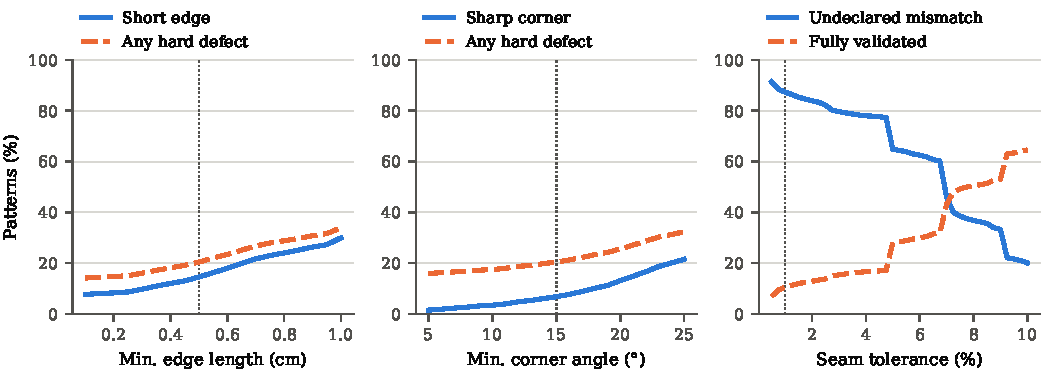
\includegraphics[width=\textwidth]{sensibilidad.pdf}
\caption{Share of neutral-body patterns flagged as each threshold is swept
with the others at their defaults (dotted line). Left and center: patterns
with the corresponding defect class and with any hard defect. Right: patterns
with an undeclared mismatch in the error zone, and patterns that are fully
validated.}
\label{fig:sens}
\end{figure*}

A short edge in a net pattern could also be a near-duplicate vertex that CAD
software would merge on import. To test this we collapse every edge shorter
than $\varepsilon$ into a single vertex at its midpoint and validate again.
Merging at $\varepsilon = 0.05$\,cm and $0.1$\,cm leaves 20.1\% and 19.2\% of
patterns with a hard defect; at $0.25$\,cm the share is 15.2\%. Merging up to
the threshold itself ($0.5$\,cm) removes the short-edge class by construction
and leaves 7.6\%, almost all sharp corners, but it also deletes 801 seams in
379 patterns, because many of the collapsed edges were sewn to another panel.
Most short edges are therefore not duplicate vertices. A fabrication pipeline
could clean part of them, but only by editing the seam graph as well.
% research/fusion_vertices.py -> figs/fusion.json

\subsection{Precision audit}
\label{sec:res-audit}

The margins and sweeps above bound how much the counts depend on threshold
values. They do not show that a reported finding is a real defect. For that we
drew a stratified random sample of 100 findings from the neutral-body corpus
with a fixed seed: 30 short edges, 30 sharp corners, 30 undeclared mismatches,
5 self-intersections and 5 panels wider than the roll. Each is rendered with
the offending element highlighted and judged by hand as a defect or a false
positive.
\todo{Precision per class after the manual audit of docs/auditoria/auditoria.csv
(research/muestra\_auditoria.py). The verdict column is empty and must be
filled by the author or a patternmaker.}
% research/muestra_auditoria.py data/garmentcodedata_0 docs/auditoria


\begin{table}[t]
\centering
\small
\setlength{\tabcolsep}{4pt}
% research/numeros_paper.py: una fila por hallazgo, cuerpo neutro
\begin{tabular}{lrrrr}
\toprule
Finding & Limit & Median & p10 & Min \\
\midrule
Sharp corner & $15^\circ$ & $11.2^\circ$ & $4.5^\circ$ & $0.12^\circ$ \\
Short edge & $0.5$\,cm & $0.15$\,cm & $0.075$\,cm & $0.018$\,cm \\
Seam mismatch & $1\%$ & $5.6\%$ & $1.7\%$ & $1.0\%$ \\
\bottomrule
\end{tabular}
\caption{Reported values against the threshold that reports them, over all
findings of each class in the neutral-body corpus (836 corners, 1{,}921 edges,
17{,}496 mismatches in the 1--15\% error zone).}
\label{tab:margins}
\end{table}

\subsection{Naive filtering collapses the corpus}
\label{sec:res-filter}

The obvious application of a validator to training data is to keep the patterns
that pass and discard the rest. On this corpus that retains 362 of 3{,}450
patterns, and the survivors are systematically simpler: a median of 6 panels
and 14 seams against 10 and 30 for the rejected. The median share of curved
edges is 25\% in both groups, so the filter selects on size and leaves shape
alone.

Complex garments are not worse made. Figure~\ref{fig:accum} plots the fully
validated rate against seam count together with the rate predicted if defects
were independent across seams. The \emph{per-seam} error rate is flat and
declines slightly with garment size, from 0.264 in patterns under ten seams to
0.177 above fifty-five. A binary per-pattern filter therefore selects against
size by construction, because a garment with thirty opportunities to fail
usually takes one.

\begin{figure}[t]
\centering
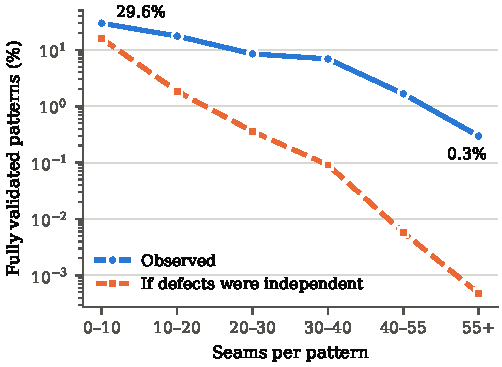
\includegraphics[width=\columnwidth]{acumulacion.pdf}
\caption{Fully validated rate by seam count (log scale): observed, and
predicted by a null model in which each seam fails independently at its bin's
per-seam error rate.}
\label{fig:accum}
\end{figure}

The gap between the two curves carries information of its own. The dashed curve is a
null model in which each seam of a pattern fails independently with probability
equal to its bin's per-seam error rate, evaluated at the bin's median seam
count $m$: the expected fully validated rate is $(1 - r)^m$. Garments with
20--30 seams have $r = 0.209$ and $m = 24$, so the null model predicts 0.36\%
fully validated; the observed rate is 8.5\%, about 24 times higher. The model
is an approximation, since $r$ counts errors, including panel-level ones,
rather than failed seams, and a seam carries at most one mismatch. Its
qualitative verdict is robust to that: some patterns are systematically good
and others systematically bad, so a per-pattern quality signal exists, and the
binary filter confounds it with size.
% research/figuras_paper.py, figura_acumulacion: pred = (1 - r)^mediana

Figure~\ref{fig:filters} compares filtering criteria by what they do to the
garment-type composition of the corpus. Discarding only hard geometric defects
retains 79.6\% of the data and leaves the composition nearly intact (full-body
garments 60.3\%\,$\rightarrow$\,58.2\%), whereas the zero-error filter retains
10.5\% and halves the full-body share to 31.5\%. Rate-based filters fall in
between: keeping patterns with at most 0.10 errors per seam retains 25.8\% of
the corpus with 48.1\% full-body garments, and a limit of 0.05 retains 13.2\%
with 37.5\%. Every criterion that counts undeclared mismatches inherits the
size bias, because those mismatches are the bulk of the errors and they
accumulate with seam count.

\begin{figure}[t]
\centering
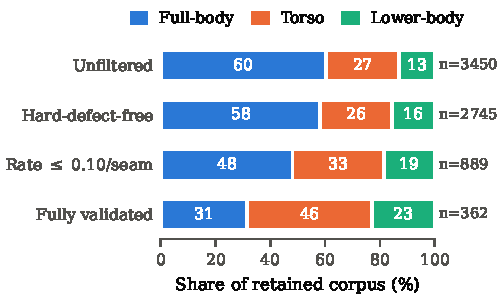
\includegraphics[width=\columnwidth]{filtros.pdf}
\caption{Garment-type composition of the neutral-body corpus retained by four
filtering criteria; $n$ is the number of patterns retained.}
\label{fig:filters}
\end{figure}

\subsection{Body shape does not affect hard-defect rates}
\label{sec:res-body}

GarmentCodeData renders each design on a neutral body and on randomized bodies.
A plausible hypothesis is that made-to-measure fitting degenerates at the
extremes of the body distribution, narrowing panels until they are uncuttable.
It does not. Aggregates are nearly identical: 20.4\% against 21.2\% of patterns
with a hard defect, and $0.195$ against $0.198$ errors per seam.

Aggregates can hide an effect when the two groups contain different designs, so
we compare \emph{paired} over the 2{,}953 designs present in both, which holds
the design fixed and varies only the body. Here a design counts as defective
if it carries a hard geometric defect. Of the 2{,}953 designs, 2{,}248 are
hard-defect-free on both bodies and 424 defective on both; the discordant cases
split 139 (defective only on the randomized body) against 142 (only on the
neutral body). An exact McNemar test gives $p = 0.91$, and the paired
difference in defect rate (randomized minus neutral) is $-0.1$ percentage
points with a 95\% confidence interval of $[-1.2, 1.0]$: no detectable
asymmetry, and any effect the data allow is small.
% research/numeros_paper.py, pareado(): IC de Wald para la diferencia pareada
% Los 705 = 139 + 142 + 424 disenos pareados coinciden por azar con los 705
% patrones con defecto duro del cuerpo neutro completo: de estos, 566 estan en
% el conjunto pareado y 139 no.

The marginal defect rates on the paired designs are 19.2\% (neutral) and
19.1\% (randomized). If the body determined which designs failed, the two
outcomes would be close to independent, and a design would be defective on
both bodies about $2{,}953 \times 0.192 \times 0.191 \approx 108$ times. It is
defective on both 424 times, 3.9 times as often. The defects come with the
parametric design and survive the change of body. They are therefore
reproducible and fixable at source, and corpus sanitization need not weight by
body type.

\subsection{Opening girths}
\label{sec:res-wear}

We ran the girth measurement of Section~\ref{sec:wear} over the corpus. Under
the default orientation all 3{,}450 patterns assemble into a coherent
free boundary, with a median of four openings per garment. The smallest opening
of a garment has a median girth of 53.4\,cm (10th percentile 25.9\,cm), and in
171 patterns (5.0\%) it is shorter than the 21\,cm hand girth of our reference
body. Whether any of these is a defect depends on what the opening must admit,
whether it has a closure and how far the fabric stretches there, and no corpus
pattern declares any of the three. We therefore report girths and issue no
wearability verdict.

\subsection{Hard defects in generated patterns}
\label{sec:res-gen}

The corpus measurement bounds what a model trained on it can learn. The
complementary question is what a model actually emits. Table~\ref{tab:generated}
reports AIpparel on the 100 paired garments of Section~\ref{sec:setup}.

\begin{table}[t]
\centering
\small
\setlength{\tabcolsep}{3pt}
\begin{tabular}{@{}lrrrr@{}}
\toprule
& \shortstack[r]{Hard-\\defect-free} & \shortstack[r]{Fully\\validated}
& Seams & \shortstack[r]{Mismatched\\seams} \\
\midrule
AIpparel (image) & 23\,/\,100 & 0\,/\,100 & 31.6 & 88\% \\
AIpparel (text)  & 17\,/\,100 & 0\,/\,100 & 26.8 & 86\% \\
Corpus & 78\,/\,100 & 12\,/\,100 & 31.5 & 33\% \\
\bottomrule
\end{tabular}
\caption{Generated patterns against the corpus patterns they were conditioned
on (ground truth), 100 garments per row.
 Seams: mean seam count per pattern. Mismatched
seams: fraction of seams whose two sides differ in length by more than 1\%
with no declared ease, including those above the 15\% gather threshold.}
\label{tab:generated}
\end{table}

Image conditioning yields 23\% hard-defect-free patterns and text
conditioning 17\%, against 78\% for the corpus patterns the model was asked to
reproduce. Full validation is stricter still: none of the 200 generated
patterns passes it, against 12 of the 100 corpus patterns. With zero successes
in 200 trials, the exact one-sided 95\% upper bound (Clopper--Pearson) on the
generated fully validated rate is 1.5\%, and the two-sided 95\% interval
reaches 1.8\%.

A count of errors per pattern rewards whichever model emits fewer seams, so it
cannot be compared across groups. The fraction of mismatched seams can.
AIpparel produces patterns with as many seams as the corpus (31.6 against
31.5), and 88\% of them are mismatched, against 33\% in the corpus.
\todo{Magnitude of the mismatch per seam (median, p25, p75 and fraction above
15\%) for the three groups. Needs AIpparel's 200 inference outputs, which are
not on disk; with them, extend research/aipparel\_contraste.py.}
It does not sew less, it sews worse. The architecture explains why. The two
edges of a seam are emitted as independent vertex predictions, and nothing in
the representation couples their lengths. Depicting the requested garment and
closing its seams are distinct objectives, and training targets only the
first.

The six-point gap between image conditioning (23\% free of hard defects) and
text conditioning (17\%) does not survive the paired test it invites. Of the 100
garments, 17 are hard-defect-free only from the image and 11 only from the
text, and an exact McNemar test on the 28 discordant cases gives $p = 0.345$.
The data show no effect of conditioning modality on the hard-defect rate,
consistent with the failure lying in the output head rather than in how well
the garment was understood.

Two cautions attach to these numbers. The descriptions are synthetic, derived
from design parameters rather than written by a person. Were they worse than
natural language, that would penalize the text condition, and it is the text
condition that showed no difference. More importantly, AIpparel was trained on
GarmentCodeData and these garments are drawn from it, so if they appeared in its
training set, these rates are a best case for the model.


\section{Discussion}

\paragraph{Upstream use.} The obvious application is the repair loop: return
localized findings to the generator and let it edit the offending site, as a
code model does with compiler diagnostics. We expect the larger effect on
training data. A corpus of 115{,}000 garments with this defect profile teaches
those defects as correct construction, and Section~\ref{sec:res-filter} shows
that cleaning it takes care, since the zero-error filter removes the defects
and most of the complex garments with them.

\paragraph{Validation rates as a metric.} The hard-defect-free and fully
validated fractions are comparable across papers, reproducible and GPU-free,
and the field does not report them. They belong next to the geometric
reconstruction metrics these systems already publish, and
Section~\ref{sec:res-gen} shows the two cannot stand in for each other. A model
can place panels that reconstruct the target garment well and still leave
nearly every seam mismatched, because no reconstruction metric is sensitive to
whether two edges that must be sewn together have the same length. We also
suggest reporting the fraction of mismatched seams, which is comparable across
models of different output complexity; per-pattern fractions are not.

\paragraph{Format and checker.} Three of our contributions are format
extensions. In Table~\ref{tab:breakdown}, two thirds of the patterns cannot be
judged because a field is missing, and no amount of checking would resolve
them.

\section{Limitations}
\label{sec:limitations}

\paragraph{Thresholds are uncalibrated.} The default limits are physically
plausible but have not been contrasted against real fabric by a professional
patternmaker. They are an explicit hypothesis. The relative claim, that
published patterns contain defects nobody checks for, does not depend on the
exact values: Figure~\ref{fig:sens} shows the hard-defect share stays between
14\% and 33\% across the swept ranges. The absolute counts should still be read
as threshold-conditional, the split between full validation and undeclared
intent depends strongly on the seam tolerance, and the precision of each
finding class awaits the manual audit of Section~\ref{sec:res-audit}.

\paragraph{Three batches of 36.} The detailed analyses use both body variants
of one batch. We repeated the headline measurement on the neutral body of two
more batches (3{,}414 and 3{,}430 patterns), streaming each archive without
storing it. The share with a hard defect is 20.4\%, 19.6\% and 20.0\% across
the three batches, and the fully validated share 10.5\%, 11.2\% and 10.5\%.
This is evidence of homogeneity, not a measurement of the whole corpus.
% research/sanear_corpus.py <destino> 1-2 ; lotes 1 y 2, cuerpo neutro


\paragraph{No downstream demonstration.} We describe the validator's use as a
filter, a repair signal and a training reward, and we characterize how
filtering should be done, but we do not report a trained model that uses it.
Establishing that a correctly filtered corpus improves a downstream generator
is the natural next experiment and is not claimed here.

\paragraph{Coverage and inference.} Assembly checking reports the cost of
sewing in the round rather than true feasibility, which is a question of
physical access and requires 3D. Drape, tension maps and dynamic poses are
outside this work entirely; we deliberately do not report simulated verdicts,
since without measured fabric parameters they would assert something unverified.
Wearability verdicts need \code{fits}, \code{stretch} and closure
declarations that no existing pattern carries, so Level~2 is evaluated here
only as girth measurement. Finally, continuity findings are a lower bound
wherever \code{orient} is undeclared, which on existing corpora is everywhere.

\paragraph{A single generator.} The corpus measurements
are on GarmentCode output and the generative measurement is on a single AIpparel
checkpoint over 100 garments, so Table~\ref{tab:generated} is a measurement, not
a ranking. Extending it to a parameter-emitting model such as ChatGarment is not
symmetric work: its outputs must pass through GarmentCode before they can be
validated, so the resulting number characterizes the model-plus-synthesizer pair
rather than the model. We can bound the second term. We passed the
\emph{ground-truth} design parameters of the same 100 garments through
GarmentCodeRC, the refined GarmentCode fork that ChatGarment ships with. The
result reproduces the published pattern's verdict on 99 of 100 garments, its
hard-defect status on 98, and its exact error count on 90. In aggregate the
synthesizer moves the fully validated rate from 12\% to 13\%, an offset of
about one percentage point. A parameter-emitting model should therefore be
scored against this reconstruction baseline rather than against the published
corpus. Our remaining claims about the expressive ceilings of these
architectures are structural, drawn from reading their code.

\section{Conclusion}

Generative garment systems are evaluated on a property that does not imply the
one industry needs. Measured on the field's own pre-training corpus, one in
five published patterns carries a hard geometric defect, and two thirds more
cannot be judged because the format does not record whether a seam mismatch
was wanted.
We release a deterministic, CPU-only validator, three format extensions that
make that intent expressible, and the benchmarks behind these numbers.

The same measurement applied to a released model finds 23\% (image) and 17\%
(text) of its patterns hard-defect-free, against 78\% of the corpus garments
it was asked to reproduce, and none fully validated, at the same seam
complexity as the corpus it was trained on. The failure is specific: edges
that must be sewn together are predicted independently and do not end up the
same length.

Two findings bear on how such a tool is used. Filtering a training corpus on
``no errors'' mostly keeps small garments, while filtering on hard geometric
defects keeps more than seven times the data and leaves the distribution
intact. And the defects follow the design program and do not change with the
body it is fitted to, so they can be reproduced and fixed where they are
introduced.



\paragraph{Availability.} \hilvan, its tests, sweep tool and figure scripts are
available under the MIT license at
\url{https://github.com/Camilo-neck/fashion-validator}.

\bibliographystyle{plainnat}
\bibliography{refs}

\appendix
\section{Implementation Notes}
\label{app:impl}

\paragraph{Self-intersection.} Validation takes 11.0\,ms and 8.3\,ms on our two
reference garments. Reaching that required one optimization:
self-intersection testing was 96\% of runtime, because the second edge was
re-linearized inside the first edge's loop and all edge pairs were compared
irrespective of proximity. We now linearize each edge once and reject pairs by
bounding box. The boxes are dilated by the vertex tolerance before comparison,
so the rejection can only do redundant work and never misses a crossing.
Every edge, arcs included, is linearized with 48 samples before the test.
GarmentCode does the same for arcs, citing an open issue in the arc
intersection routine of svgpathtools~\citep{svgpathtools121}, the geometry
library both implementations use.


\paragraph{Running AIpparel on 16\,GB.} The released checkpoint is stored in
fp32 while the model instantiates in bf16, so loading it with
\code{torch.load} materializes 25\,GiB of anonymous memory. Memory-mapping the
file keeps the resident set under 1.5\,GiB and lets inference run on a single
16\,GB GPU.


\end{document}
